\documentclass[landscape]{beamer}

\usepackage[utf8]{inputenc}
\usepackage{graphicx}
\usepackage{booktabs}
\usepackage{stmaryrd}
\usepackage{extarrows}
% \usepackage[colorlinks=true,linkcolor=blue,urlcolor=black]{hyperref}
\usepackage{hyperref}
\usepackage{bookmark}
\usepackage{tikz}
\usetikzlibrary{automata, positioning, shapes.misc}

\mode<presentation> {
\usetheme{Madrid}
% \usetheme[width=0]{Berkeley}
% \usetheme{Luebeck}

% \useinnertheme{circles}
\useinnertheme{rectangles}

\usefonttheme{professionalfonts}
}

\AtBeginSection[]
{
\begin{frame}
\frametitle{Contents}
\tableofcontents[currentsection]
\end{frame}
}

\title{Cost Register Automata}
% \author{Abreto Fu}
% \institute{Institute of Software}
\date{2019.12.20}

\newcommand{\op}{\mathit{op}}
\newcommand{\setQ}{\mathbb{Q}}
\newcommand{\calO}{\mathcal{O}}
\newcommand{\calA}{\mathcal{A}}
\newcommand{\bbE}{\mathbb{E}}
\newcommand{\ttVal}{\mathtt{val}}
\newcommand{\val}{\ttVal}
\newcommand{\setN}{\mathbb{N}}
\newcommand{\sfR}{\mathsf{R}}
\newcommand{\sem}[1]{\llbracket {#1} \rrbracket}
\newcommand{\dom}{\mathrm{dom}}
\newcommand{\calP}{\mathcal{P}}
\newcommand{\eps}{\varepsilon}

\begin{document}

% \pdfbookmark{Title}{Title}
\frame{\titlepage}

% \pdfbookmark{Contents}{Contents}
\begin{frame}{Overview}
    \tableofcontents
\end{frame}

\section{Introduction}
\begin{frame}
\frametitle{Introduction}
% \begin{block}{Function}
% A CRA processes a data word (a sequence over $\Sigma\times D$)
% and outputs a value in $D$
% that is computed using a given set of operations over $D$.
% \end{block}
% \begin{block}{Goals}
% \begin{itemize}
%     \item Providing a machine-based characterization of
%     the class of \textit{regular transductions}
%     from strings to costs.
% \end{itemize}
% \end{block}
\begin{block}{A Cost Register Automaton (CRA)}
\begin{itemize}
    \item process a data word (a sequence of tagged values)
        and outputs a value in a data set
        that is computed using a given set of operations over the data set;
    \item provides a machine-based characterization
    of the class of \textit{regular transductions} from strings to costs.
\end{itemize}
\end{block}
\end{frame}

\section{Data Transductions}
\newcommand{\sigxd}{\Sigma \times D}
\newcommand{\tagproj}{|_\Sigma}
\begin{frame}{Data Transductions}
    \begin{block}{Notations}
    \begin{itemize}
        \item $\Sigma$ is a finite alphabet whose elements are called \alert{tags};
        \item $D$ is a data set of \alert{data values}.
    \end{itemize}
    \end{block}
    
    \pause

    \begin{definition}
    A \alert{data word} is a sequence of tagged values,
    i.e. a word over the alphabet $\Sigma \times D$.
    \end{definition}
    \pause
    \begin{example}
        Suppose $\Sigma = \{ a, \# \}, D = \setN$. Then
        \[ (a,0)(a,2)(\#,0)(a,1)(\#,2) \]
        is a data word.
    \end{example}
\end{frame}
\begin{frame}{Data Transductions}
    \begin{definition}
    A \alert{data transduction} is a partial function of type
    \[ (\Sigma \times D)^* \rightharpoonup D. \]
    \end{definition}
    \pause
    
    \begin{definition}
    A multi-valued transduction is a partial function of type
    \[ (\sigxd)^* \to \mathcal{P}(D), \]
    where $\calP$ is the powerset operator.
    \end{definition}
    
    % \begin{block}{Notations}
    % \begin{itemize}
    %     \item $\calO$ is a family of constants and operations
    %         that are allowed on the data set $D$;
    %     \item $\calO_n$ denotes the set of $n$-ary operations
    %         that are contained in $\calO$;
    %     \item $\calO_0$ is the set of constants in $\calO$, in particular.
    % \end{itemize}
    % \end{block}
\end{frame}
\begin{frame}{Data Transductions}
    \begin{definition}
    For a data word $w \in (\sigxd)^*$,
    $w|_\Sigma$ denotes the elementwise projection of $w$ to the tag component.
    Formally,
    \[
        (a_1, d_1)(a_2, d_2)\cdots(a_n, d_n)\tagproj = a_1a_2 \cdots a_n
    \]
    \end{definition}
    \pause
    
    \begin{definition}
    The \alert{rate} of $f$ is the language $\sfR(f) \subseteq \Sigma^*$
    defined as follows:
    \[
    \sfR(f) = 
        \{ \sigma \in \Sigma^* |
            \forall w \text{ with } w\tagproj = \sigma,
            f(w) \text{ is defined}
        \}.
    \]
    \end{definition}
\end{frame}

\section{Syntax and Semantics of CRAs}
\begin{frame}{Syntax and Semantics of CRAs}
    \begin{block}{Notations}
    \begin{itemize}
        \item $X$ is a set of variables;
        \item $\calO$ is a family of constants and operations
            that are allowed on the data set $D$;
        \begin{itemize}
            \item $\calO_n$ denotes the set of $n$-ary operations
                that are contained in $\calO$;
            \item $\calO_0$ is the set of constants in $\calO$, in particular.
        \end{itemize}
    \end{itemize}
    \end{block}
    \pause
    \begin{definition}
    $\bbE_\calO[X]$ denotes the set of \alert{expressions} over $X$,
    defined by the following rules:
    \begin{itemize}
        \item $c \in \bbE_\calO[X]$, if constanc $c \in \calO$;
        \item $x \in \bbE_\calO[X]$, if variable $x \in X$;
        \item $op(t_1, \dots, t_n) \in \bbE_\calO[x]$,
            if $n$-ary operation $op \in \calO$,
            $t_i \in \bbE_\calO[X]$ for all $i = 1, \dots, n$.
    \end{itemize}
    \end{definition}
\end{frame}
\begin{frame}{Syntax and Semantics of CRAs}
    \begin{definition}[CRA]
    A (nondeterministic, copyful) \alert{Cost Register Automaton (NCRA)}
    over the tag alphabet $\Sigma$, data values $D$,
    and data operations $\calO$ is a tuple
    \[
        \calA = (Q, X, \Delta, I, F),
    \]
    where
    \begin{itemize}
        \item $Q$ is a finite set of states,
        \item $X$ is a finite set of registers,
        \item $\Delta \subseteq Q \times \Sigma \times U_\calO \times Q$ is the set of 
            transitions with $U_\calO$ the set of register updates
            $X \to \bbE_\calO[X \cup \{ \ttVal \}]$,
        \item $I: Q \rightharpoonup (X \to \bbE_\calO[\emptyset])$ is the initialization function, and
        \item $F: Q \rightharpoonup \bbE_\calO[X]$ is the finalization function.
    \end{itemize}
    \end{definition}
\end{frame}
\begin{frame}{Syntax and Semantics of CRAs}
    \begin{block}{Branches}
    \centering
    \begin{tabular}{r|ccc}
        abbreviations & NCRA & UCRA & DCRA \\\hline
        the automaton is & nondeterministic & unambiguous & deterministic
    \end{tabular}
    \end{block}
    \pause
    
    \begin{definition}
    A CRA is said to be \alert{copyless} if
    \begin{enumerate}
        \item $\forall (p,a,\theta,q) \in \Delta, \forall x \in X$,
            there is at most one occurrence of $x$ in the list of expressions
            $\theta(x_1),\dots,\theta(x_n)$,
            where $x_1,\dots,x_n$ is an enumeration of $X$, and
        \item $\forall q \in \dom(F), \forall x \in X$,
            there is at most one occurrence of $x$ in the expression $F(q)$.
    \end{enumerate}
    \end{definition}
\end{frame}

\begin{frame}{Syntax and Semantics of CRAs}
    \begin{definition}
    A function $\alpha: X \to D$ is called a \alert{variable assignment}.
    It extends uniquely to a homomorphism $\hat{\alpha}: \bbE_\calO[X] \to D$.
    \end{definition}
    \pause
    
    \begin{block}{Notations}
    \begin{itemize}
        \item \texttt{val} is a special symbol,
            referring to the value of the current data item;
        \item $\alpha[\ttVal \mapsto d]$ means the extension of $\alpha$
            that maps \texttt{val} to $d$.
    \end{itemize}
    \end{block}
    \pause

    \begin{definition}
    An expression $t \in \bbE_\calO[X]$ denotes a function $\sem{t}: D^X \to D$,
    defined as:
    \begin{quote}
        for a variable assignment $\alpha: X \to D$,
        put $\sem{t}(\alpha) = \hat{\alpha}(t)$.
    \end{quote}
    \pause
    
    An expression $t \in \bbE_\calO[X \cup \{\ttVal\}]$
        denotes a function $\sem{t}: D^X \times D \to D$,
    \[
        \sem{t}(\alpha, d) = \hat{\beta}(t) \text{ where }
            \beta = \alpha[\ttVal \mapsto d]:
            X \cup \{ \ttVal \} \to D
    \]
    \end{definition}
\end{frame}

\begin{frame}{Syntax and Semantics of CRAs}
    \begin{definition}
    For an input sequence $w = (a_1,d_1)(a_2,d_2)\cdots(a_n,d_n) \in (\sigxd)^*$,
    we define a \alert{$w$-run} in $\calA$ to be a sequence
    \[
        (q_0,\alpha_0)
        \xlongrightarrow{(a_1,d_1)} (q_1,\alpha_1)
        \xlongrightarrow{(a_2,d_2)} (q_2,\alpha_2)
        \xlongrightarrow{(a_3,d_3)} \cdots
        \xlongrightarrow{(a_n,d_n)} (q_n,\alpha_n)
    \]
    with $q_i \in Q$ and $\alpha_i: X \to D$ for all $i$ so that:
    \begin{enumerate}
        \item \textit{Initialization:}
            $q_0 \in \dom(I)$ and
            $\alpha_0(x) = \sem{I(q_0)(x)}$ for every register $x \in X$;
        \item \textit{Transition:}
            $\forall (p,\alpha)\xlongrightarrow{(a,d)}(q,\beta)$,
            $\exists \theta \in U_\calO \text{ with } (p,a,\theta,q) \in \Delta$ s.t.
            \[
                \forall x \in X, \: \beta(x) = \sem{\theta(x)}(\alpha, d);
            \]
        \item \textit{Finalization:}
            $q_n \in \dom(F)$.
    \end{enumerate}
    
    The \alert{value} of the run is $\sem{F(q_n)}(\alpha_n)$.
    \end{definition}
\end{frame}

\section{Examples}
\begin{frame}{Example 1}
    \begin{block}{Suppose}
        $\Sigma = \{a, b\}, D = \setN, \calO = \{0, +\}$
    \end{block}
    \begin{block}{Transduction}
    \[ f: (\sigxd)^* \rightharpoonup D, \text{ defined on all nonempty sequences.} \]
    If a sequence ends with an $a$-labeled ($b$-labeled) value,
    then $f$ outputs the sum of all $a$-labeled ($b$-labeled) values in the sequence.
    \end{block}
\end{frame}
\begin{frame}{Example 1}
    \begin{block}{Copyless DCRA}
    \begin{gather*}
        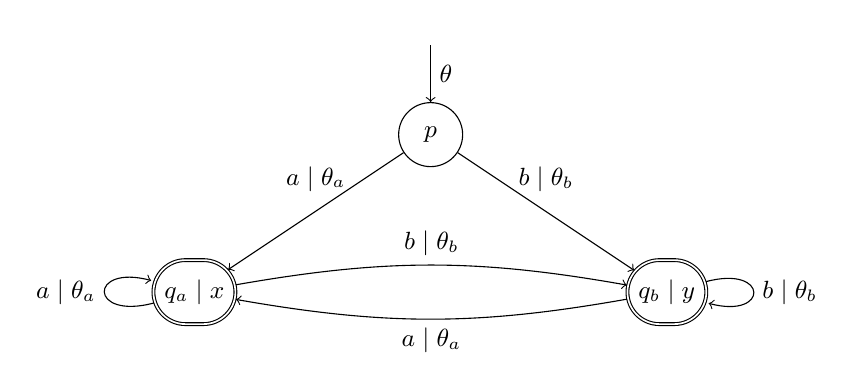
\begin{tikzpicture}[node distance=3cm, ->]
        \small
        %
        \node (i) {};
        \node [state, below of=i, node distance=1.25cm] (p) {$p$};
        \node [below of=p, node distance=2cm] (p2) {};
        \node [state, accepting, rounded rectangle, left of=p2] (qa) {$q_a \mid x$};
        \node [state, accepting, rounded rectangle, right of=p2] (qb) {$q_b \mid y$};
        %
        \path (i) edge node[right] {$\theta$} (p);
        \path (p) edge node[above, yshift=1ex] {$a \mid \theta_a$} (qa);
        \path (p) edge node[above, yshift=1ex] {$b \mid \theta_b$} (qb);
        \path (qa) edge[loop left] node[left] {$a \mid \theta_a$} (qa);
        \path (qb) edge[loop right] node[right] {$b \mid \theta_b$} (qb);
        \path (qa) edge[bend left=10] node[above] {$b \mid \theta_b$} (qb);
        \path (qb) edge[bend left=10] node[below] {$a \mid \theta_a$} (qa);
        \end{tikzpicture}
    \end{gather*}
    \begin{align*}
    \theta &= \begin{cases}
      x := 0 \\
      y := 0
    \end{cases}
    &
    \theta_a &= \begin{cases}
      x := x + \ttVal \\
      y := y
    \end{cases}
    &
    \theta_b &= \begin{cases}
      x := x \\
      y := y + \ttVal
    \end{cases}
    \end{align*}
    \end{block}
\end{frame}

\begin{frame}{Example 2}
    \begin{block}{Copyless UCRA}
    \begin{gather*}
    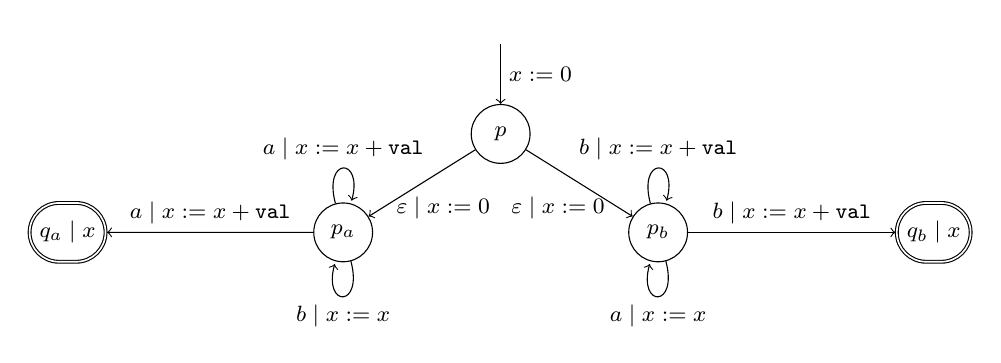
\begin{tikzpicture}[node distance=3.5cm, ->]
    \footnotesize
    %
    \node (i) {};
    \node [state, below of=i, node distance=1.25cm] (p) {$p$};
    \node [below of=p, node distance=1.25cm] (p2) {};
    \node [state, left of=p2, node distance=2.0cm] (pa) {$p_a $};
    \node [state, accepting, rounded rectangle, left of=pa] (qa) {$q_a \mid x$};
    \node [state, right of=p2, node distance=2.0cm] (pb) {$p_b$};
    \node [state, accepting, rounded rectangle, right of=pb] (qb) {$q_b \mid x$};
    %
    \path (i) edge node[right] {$x := 0$} (p);
    \path (p) edge node[below, pos=0.3, yshift=-2ex] {$\eps \mid x := 0$} (pa);
    \path (p) edge node[below, pos=0.3, yshift=-2ex] {$\eps \mid x := 0$} (pb);
    \path (pa) edge[loop above] node[above] {$a \mid x := x + \val$} (pa);
    \path (pa) edge[loop below] node[below] {$b \mid x := x$} (pa);
    \path (pa) edge node[above] {$a \mid x := x + \val$} (qa);
    \path (pb) edge[loop above] node[above] {$b \mid x := x + \val$} (pb);
    \path (pb) edge[loop below] node[below] {$a \mid x := x$} (pb);
    \path (pb) edge node[above] {$b \mid x := x + \val$} (qb);
    \end{tikzpicture}
    \end{gather*}
    \end{block}
\end{frame}

\begin{frame}{Example 3}
    \begin{block}{Suppose}
    $\Sigma = \{a, \#\}$, $D = \setN$, $\calO = \{0, +, \mathrm{max}\}$.
    \end{block}
    \begin{block}{Transduction}
    \[ f: (\sigxd)^* \rightharpoonup D, \quad \text{rate: } (a^+\#)^* \]
    $f$ outputs the maximum cost over all input blocks, where
    \begin{itemize}
        \item a block is a maximal subsequence of the input
            that is of the form $aa \dots a \#$,
        \item the cost of a block is the sum of the $a$-labeled values.
    \end{itemize}
    \end{block}
\end{frame}
\begin{frame}{Example 3}
    \begin{block}{Copyless DCRA}
    \begin{gather*}
    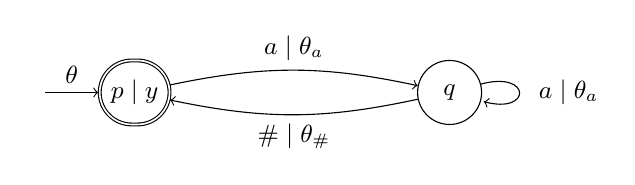
\begin{tikzpicture}[node distance=4cm, ->]
    \small
    %
    \node (i) {};
    \node [state, accepting, rounded rectangle, right of=i, node distance=1.25cm] (p) {$p \mid y$};
    \node [state, right of=p] (q) {$q$};
    %
    \path (i) edge node[above] {$\theta$} (p);
    \path (p) edge[bend left=12] node[above] {$a \mid \theta_a$} (q);
    \path (q) edge[bend left=12] node[below] {$\# \mid \theta_\#$} (p);
    \path (q) edge[loop right] node[right, xshift=1ex] {$a \mid \theta_a$} (q);
    \end{tikzpicture}
    \end{gather*}
    \begin{align*}
    \theta &= \begin{cases}
      x := 0 \\
      y := 0
    \end{cases}
    &
    \theta_a &= \begin{cases}
      x := x + \val \\
      y := y
    \end{cases}
    &
    \theta_\# &= \begin{cases}
      x := 0 \\
      y := \max(y,x)
    \end{cases}
    \end{align*}
    \end{block}
\end{frame}

\begin{frame}{Example 4}
    \begin{block}{Suppose}
    $\Sigma = \{a,b\}, D = \setN, \calO = \{0, \ominus\}$.
    $x \ominus y = \mathrm{max}(x - y, 0)$.
    \end{block}
    \begin{block}{Transduction}
    \[ f: (\sigxd)^* \rightharpoonup D, \]
    defined on sequences that contain at least one $a$-labeled value.
    
    $f$ outputs the maximum drawdown in the input signal
    after the last occurrence of a $b$-labeled value.
    \end{block}
\end{frame}
\begin{frame}{Example 4}
    \begin{block}{Copyful UCRA}
    \begin{gather*}
    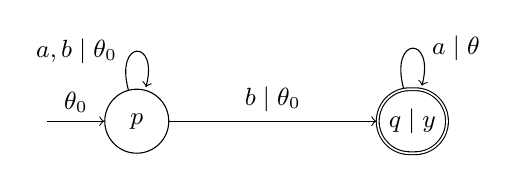
\begin{tikzpicture}[node distance=3.5cm, ->]
    \small
    %
    \node (i) {};
    \node [state, right of=i, node distance=1.25cm] (p) {$p$};
    \node [state, accepting, rounded rectangle, right of=p] (q) {$q \mid y$};
    %
    \path (i) edge node[above] {$\theta_0$} (p);
    \path (p) edge node[above] {$b \mid \theta_0$} (q);
    \path (p) edge[loop above] node[left, xshift=-1ex] {$a,b \mid \theta_0$} (p);
    \path (q) edge[loop above] node[right, xshift=1ex] {$a \mid \theta$} (q);
    \end{tikzpicture}
    \end{gather*}
    \begin{align*}
    \theta_0 &= \begin{cases}
      x := 0 \\
      y := 0
    \end{cases}
    &
    \theta &= \begin{cases}
      x := \max(x, \val) \\
      y := \max(y, \max(x, \val) \ominus \val)
    \end{cases}
    \end{align*}
    \end{block}
\end{frame}

\begin{frame}{Example 5}
    \begin{block}{Suppose}
    $\Sigma = \{a\}, D = \setQ, \calO = \{0, op\}$.
    \[ op(x,y) = \lambda \cdot x + y, \quad \lambda \in (0,1). \]
    \end{block}
    \begin{block}{Transduction}
    For $w$ with $w|_D = d_1d_2\dots d_n \in D^*$,
    $f$ outputs
    \[
        \lambda^{n-1} \cdot d_1 + \cdots + \lambda \cdot d_{n-1} + d_n.
    \]
    \end{block}
\end{frame}
\begin{frame}{Example 5}
    \begin{block}{CRA}
    \begin{gather*}
    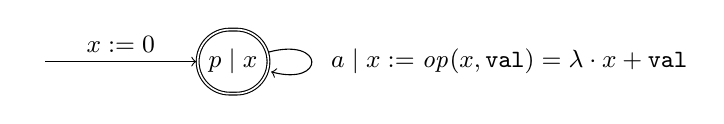
\begin{tikzpicture}[node distance=4cm, ->]
    \small
    \node (i) {};
    \node [state, accepting, rounded rectangle, right of=i, node distance=2.5cm] (q) {$p \mid x$};
    \path (i) edge node[above] {$x := 0$} (q);
    \path (q) edge[loop right] node[right, xshift=1ex] {$a \mid x := \op(x, \val) = \lambda \cdot x + \val$} (q);
    \end{tikzpicture}
    \end{gather*}
    \end{block}
\end{frame}

\begin{frame}{Example 5}
    \begin{block}{Transduction}
    \[ g(w_1w_2 \dots w_n) = f(w_n  \dots w_2w_1). \]
    \end{block}
    \pause
    \begin{block}{CRA with a hole}
    \begin{gather*}
    \begin{tikzpicture}[node distance=4cm, ->]
    \small
    \node (i) {};
    \node [state, accepting, rounded rectangle, right of=i, node distance=3cm] (q) {$p \mid x[0/\Box]$};
    \path (i) edge node[above] {$x := \Box$} (q);
    \path (q) edge[loop right] node[right, xshift=1ex] {$a \mid x := x[\op(\Box,\val)/\Box]$} (q);
    \end{tikzpicture}
    \end{gather*}
    $x[t/\Box]$ denotes the result of
    substituting $t$ for $\Box$ in the term that $x$ holds.
    \end{block}
\end{frame}

\end{document}
